\documentclass[letterpaper,10pt,twoside,twocolumn,openany]{book}
\usepackage[layout=true,bg=full]{dnd} % this has to come first in order for this to work
\usepackage{dndnotes}
\usepackage{listings}
\usepackage[english]{babel}
\usepackage[utf8]{inputenc}
\usepackage{pgfplots} 
\usepackage{amsmath}
\usepackage{wallpaper}
\usepackage{cancel}
\usepackage{mathtools}
\usepackage{polynom}
\usepackage[hidelinks]{hyperref}
\usepackage{amsthm,amssymb}
\usepackage{appendix}
\usepackage{datetime}
\usepackage{subfiles}
\usepackage{comment}
\usepackage{microtype}
\usepackage{lmodern}
\usepackage{geometry,graphicx,theorem}
\usepackage{tasks}
\pgfplotsset{compat=1.15}

\colorlet{tablecolor}{PhbLightCyan}
 

% Note that book class by default is formatted to be printed back-to-back.
\begin{document}                       
\frontmatter                           
\begin{titlepage}
  \begin{tikzpicture}[remember picture,overlay]
    \node[inner sep=0pt] at (current page.center) {
\includegraphics[width=\paperwidth,height=\paperheight]{./cover.jpg}};
  \end{tikzpicture}~
    \newpage
    
    \begin{center}
        

        \large
        \vspace*{\fill}
        Master the skills of integration using the techniques listed in this book. From regular and trigonometric substitutions, partial fractions, and integration by parts. Using the right technique(s) will lead you to a heroic victory against the machination of the professor. 
        \\~\\
        By slaying his assignment minions, defeating his midterm champion(s) and ending the final themselves. The heroic legacy of your achievement will be remembered on your academic transcript.
        \\~\\
        \vspace*{\fill}

    \end{center}
    \let\thefootnote\relax\footnote{Disclaimer: Please don't use the integration symbol as a weapon, especially against an Ancient Red Dragon, or a dragon of any kind. If you do they will most certainly mock you for your stupidity before incinerating you.}
\end{titlepage}

\tableofcontents                        % Print table of contents
\mainmatter                             % only in book class (Arabic page #s)

                        
\chapter{Math 114 Review}                % Print a "chapter" heading
\section{Derivatives}
\begin{DndSidebar}{Derivative Definition}
    Let a function $f ( x)$ be defined on an open interval $I = ( a, b)$. The function $f ( x)$ is differentiable at $x_0 \in I$ if the following limit exists
    \[ f' ( x_0) = \lim_{x \rightarrow x_0} \frac{f ( x) - f ( x_0)}{x - x_0} . \]
    An equivalent formula is derived if we take $x - x_0 = h$
    \[ f' ( x_0) = \lim_{h \rightarrow 0} \frac{f ( x_0 + h) - f ( x_0)}{h} . \]
\end{DndSidebar}


\begin{description}
    \item[Geometrical Interpretation] The interpretation is shown in the
    following figure
    
    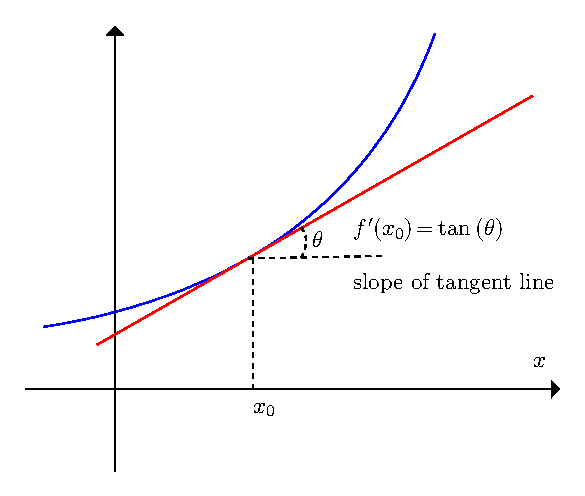
\includegraphics[scale=0.83]{supplement-1.eps}
    
    \item[Physical Interpretation] If $x = f ( t)$ denote the position of a mass particle on the $x$-axis, where $t$ stands for time, the value $f' ( t_0)$ measures the velocity of the particle at $t_0$.
    \\~\\
    If $f' ( t_0) > 0$ the particle moves forward, if $f' ( t_0) < 0$ the particle moves backward.
    \\~\\
    What is the physical interpretation of $f'' ( t)$?
\end{description}
\newpage

\subsection{Linear Approximation}
In the definition of derivative, if we relax the limit, we can write
\[ f' ( x_0) \cong \frac{f ( x) - f ( x_0)}{x - x_0}, \]
or equivalently
\[ f ( x) \cong f ( x_0) + f' ( x_0) ( x - x_0). \]
The right hand side of the above equality is just the equation of the tangent line,
\[ T ( x) = f ( x_0) + f' ( x_0) ( x - x_0), \]
thus for $x$ close to $x_0$ we obtain the following approximation
\[ f ( x) \cong T ( x). \]
\subsubsection*{Example}
Use the linear approximation to approximate $\sqrt{66}$.
\subsubsection*{Solution}
Take $f ( x) = \sqrt{x}$ and thus if we take $x_0 = 64$, we can write
\begin{gather*}
    f ( 66) \cong f ( 64) + f' ( 64) ( 66 - 64)\\
    = 8 + \frac{1}{16} ( 2) = 8 + \frac{1}{8} = \frac{65}{8} \cong 8.125 
\end{gather*} 
We see the approximate value is close to the real value of $f ( 66) = 8.1240384$.

\subsubsection*{Exercise}
Use linear approximation and approximate $\log_2 ( 2.1)$.

\newpage
\subsection{General Rules of Derivatives}
\begin{DndSidebar}{The rules for derivatives}
    These are the general rules for derivatives.
    \begin{equation}
        y = x^n \Rightarrow y' = nx^{n-1}\ dx
    \end{equation}
    \begin{equation}
        y = \sin(x) \Rightarrow y' = \cos(x)\ dx
    \end{equation}
    \begin{equation}
        y = \cos(x) \Rightarrow y' = -\sin(x)\ dx
    \end{equation}
    \begin{equation}
        y = e^x \Rightarrow y' = e^x\ dx
    \end{equation}
    \begin{equation}
        y = \ln|x| \Rightarrow y' = \frac{1}{x}\ dx
    \end{equation}
    \begin{equation}
        (fg)' = f'g + fg'
    \end{equation}
    \begin{equation}
        \left( \frac{f}{g} \right)' = \frac{f'g - fg'}{g^2}
    \end{equation}
    \begin{equation}
        (f(g(x)))' = f'(g(x)) \cdot g'(x)
    \end{equation}
    \begin{equation}
        (a^{f(x)})' = f'(x) \ln(a) 
    \end{equation}
    \begin{equation}
        y = (f(x)^{g(x)}) \Rightarrow y' = y\cdot (g(x)\cdot \ln(f(x)))'
    \end{equation}
    \begin{equation}
        y = log_a f(x) \Rightarrow y' = \frac{f(x)'}{f(x)\cdot\ln(a)}
    \end{equation}
    \begin{equation}
        \sinh(x)' = \cosh(x)
    \end{equation}
    \begin{equation}
        \cosh(x)' = \sinh(x)
    \end{equation}
\end{DndSidebar}

\section{L'Hospital's Rule}
\begin{DndSidebar}{L'Hospital's Rule}
    Suppose $f$ and $g$ are differentiable and $g'(x) \neq 0$ on an open interval $I$ that contains $a$ (except possibly at $a$). Suppose that
    \begin{gather*}
        \lim_{x\to a} f(x) = 0\ \text{and}\ \lim_{x\to a} g(x) = 0\\
        \text{or that}\\
        \lim_{x\to a} f(x) = \pm\infty\ \text{and}\ \lim_{x\to a} g(x)= \pm\infty\\
        \text{Then}\\ 
        \lim_{x\to a}\frac{f(x)}{g(x)} = \lim_{x\to a} \frac{f'(x)}{g'(x)}
    \end{gather*}
    if the limit on the right side exists (or is $\infty$ or $-\infty$).
\end{DndSidebar}
\newpage
\section{Derivatives of inverse functions}
\begin{DndSidebar}{The general formula}
    If we have an expression like this: $ y = f^{-1}(x)$. This is equivalent to:
    \begin{equation}
        y = f^{-1}(x) \Leftrightarrow f(y) = x
    \end{equation}
    The derivative of y is then:
    \begin{align*}
        (f(y))' = (x)'
    \end{align*}
    Using the chain rule we get
    \begin{align*}
        f'(y)\cdot y' &= 1\\
        y' &= \frac{1}{f'(y)}\\
        y' &= \frac{1}{f'(f^{-1}(x))}
    \end{align*}    
\end{DndSidebar}

\subsection{Inverse Trigonometric Functions}
\begin{DndSidebar}{Inverse Trigonometric Functions}
    These are the standard trigonometric functions, their inverse, and their domains.
    \begin{gather}
        \theta = \cos^{-1}(x) \Leftrightarrow x = \cos(\theta)\\ 
        \nonumber
        \theta\in [0,\pi],\ x\in[-1\leq x\leq 1]
        \nonumber\\
        \nonumber~\\  
        \theta = \sin^{-1}(x) \Leftrightarrow x = \sin(\theta)\\
        \nonumber
        \theta\in \biggl[-\frac{\pi}{2},\frac{\pi}{2}\biggl],\ x\in[-1\leq x\leq 1]
        \nonumber\\
        \nonumber~\\
        \theta = \tan^{-1}(x) \Leftrightarrow x = \tan(\theta)\\ 
        \nonumber
        \theta\in \biggl[-\frac{\pi}{2},\frac{\pi}{2}\biggl],\ x\in(-\infty, \infty)
    \end{gather}
\end{DndSidebar}
\newpage
When you have an expression in the form like this $f(g^{-1}(x))$ where $f(x)$, and $g^{-1}(x)$ are trigonometric functions then using the following equation above we get these trigonometric identities.

\begin{DndComment}{Cos inverse}
    If you have
    $
        y = \theta = \cos^{-1}(x)
    $.
    Then, representing the trigonometric function using a triangle is shown below\\
    \begin{tikzpicture}
        \node at (0,0) (A) {};
        \node at (4,0) (B) {};
        \node at (4,2) (C) {};
        \node at (1,0.25) (D) {$\theta$};
        
        \draw (0,0) -- (4,0) node [midway, below] (a) {$x$};
        \draw (0,0) -- (4,2) node [midway, above,sloped] (h) {$1$};
        \draw (4,0) -- (4,2) node [midway, right] (o) {$\sqrt{1-x^2}$}; 
        
    \end{tikzpicture}
    \begin{gather}
        \sin(\cos^{-1}(x)) = \sqrt{1-x^2}\\
        \tan(\cos^{-1}(x)) = \frac{\sqrt{1-x^2}}{x}
    \end{gather}
\end{DndComment}

\begin{DndComment}{Sin inverse}
    If you have
    $
        y = \theta = \sin^{-1}(x)
    $.
    Then, representing the trigonometric function using a triangle is shown below\\
    \begin{tikzpicture}
        \node at (0,0) (A) {};
        \node at (4,0) (B) {};
        \node at (4,2) (C) {};
        \node at (1,0.25) (D) {$\theta$};

        \draw (0,0) -- (4,0) node [midway, below] (a) {$\sqrt{1-x^2}$};
        \draw (0,0) -- (4,2) node [midway, above,sloped] (h) {$1$};
        \draw (4,0) -- (4,2) node [midway, right] (o) {$x$}; 
        
    \end{tikzpicture}
    \begin{gather}
        \cos(\sin^{-1}(x)) = \sqrt{1 - x^2}\\
        \tan(\sin^{-1}(x)) = \frac{x}{\sqrt{1 - x^2}}
    \end{gather}
\end{DndComment}

\begin{DndComment}{Tan inverse}
    If you have
    $
        y = \theta = \tan^{-1}(x)
    $.
    Then, representing the trigonometric function using a triangle is shown below\\
    \begin{tikzpicture}
        \node at (0,0) (A) {};
        \node at (4,0) (B) {};
        \node at (4,2) (C) {};
        \node at (1,0.25) (D) {$\theta$};


        \draw (0,0) -- (4,0) node [midway, below] (a) {$1$};
        \draw (0,0) -- (4,2) node [midway, above,sloped] (h) {$\sqrt{1 + x^2}$};
        \draw (4,0) -- (4,2) node [midway, right] (o) {$x$}; 
        
    \end{tikzpicture}
    \begin{gather}
        \sin(\tan^{-1}(x)) = \frac{x}{\sqrt{1 + x^2}}\\
        \cos(\tan^{-1}(x)) = \frac{1}{\sqrt{1 + x^2}}
    \end{gather}
\end{DndComment}

\newpage

\subsubsection{Example}
$$ 
    y = \tan^{-1}(x) 
$$
What is y'?
\begin{gather*}
    \tan^{-1}(x) = y \Rightarrow \tan(y) = x\\ 
    \sec^2(y)\cdot y' = 1\\ 
    y' = \frac{1}{\sec^2(y)}\\ 
    y' = \frac{1}{\sec^2(\tan^{-1}(x))}\\
    \text{From the Tan inverse box we}\\ 
    \text{know that $\sec(\theta) = \sqrt{1 + x^2}$.}\\ 
    y' = \frac{1}{\sec^2(\sqrt{1 + x^2})}\\ 
    y' = \frac{1}{1 + x^2}\ dx
\end{gather*}
\section{Implicit functions}
If you have an expression where the variable you are deriving is being used in a function or is not alone. Then you have to derive both sides of the = sign to evaluate the expression. This type of function is called an implicit as the variable in question isn't explicitly defined. 
\\~\\ 
You derive each term with respect to the variable you are deriving for and collect the deriving variable on one side and all other terms to the other,
\subsubsection{Example}
\begin{align*}
    e^y + y + x^2 + \sin(x) &= 3\\
    y' = e^y\cdot y' + y' + 2x + \cos(x) &= 0\\
    y'(e^y + 1)+ 2x + \cos(x) &= 0\\
    y' = \frac{-2x - \cos(x)}{e^y + 1}\ dx
\end{align*}
\newpage

\section{Integrals} 
\subsection{Riemann Sum}
\begin{DndSidebar}{Riemann Sum}
    Let $y = f ( x)$ and $a \leq x \leq b$ is a continuous function. The area under the curve of the function is calculated by the formula
    \[ A = \lim_{n \rightarrow \infty} \sum_{n = 1}^n f ( x_k) \Delta x, \]
    where $\Delta x = \frac{b - a}{n}$, and $x_k = a + k \Delta x$.
    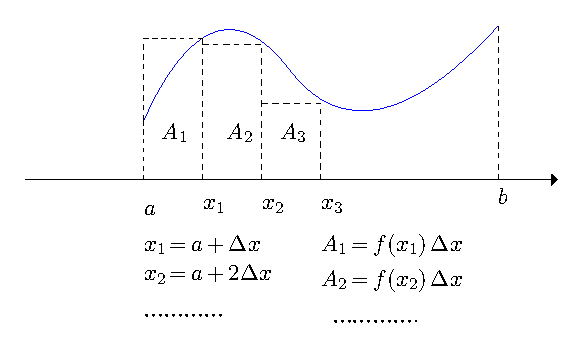
\includegraphics[scale=0.8]{supplement-2.eps}
\end{DndSidebar}
\subsection{Fundamental Theorem of Calculus}
\begin{DndSidebar}{Fundamental Theorem of Calculus}
    The fundamental theorem of calculus states that
    \[ A = \int_a^b f(x)\ dx \]
    where $\int$ stands for the anti-derivative operation.
\end{DndSidebar}
\subsubsection*{Example}
For finding the area under the curve $y = x^2$, $0 \leq x \leq 1$, we use the Riemann sum. We have $a = 0, b = 1$, and thus $\Delta x = \frac{1 - 0}{n} = \frac{1}{n}$. 
Intermediate points are $x_k = a + k \Delta x = \frac{k}{n}$, and thus
\[ A = \lim_{n \rightarrow \infty} \sum_{k = 1}^n \left( \frac{k}{n} \right)^2 \frac{1}{n} = \lim_{n \rightarrow \infty} \frac{1}{n^3} \sum_{k = 1}^n k^2 . \]
We know
\[ \sum_{k = 1}^n k^2 = \frac{n ( n + 1) ( 2 n + 1)}{6}, \]
and thus
\[ A = \lim_{n \rightarrow \infty} \frac{( n + 1) ( 2 n + 1)}{6 n^2} =
   \frac{1}{3} . \]
Alternatively, we can use the fundamental theorem of calculus and write
\[ A = \int_0^1 x^2 dx = \frac{1}{3} x^3 |_0^1 = \frac{1}{3} . \]

\subsection{General Rules for Integrals}
\begin{DndSidebar}{The general rules for integrals}
    There are two different types of integrals: indefinite and definite
    \subsubsection{Indefinite}
        \begin{equation}
            \int 1 dx = x + C
        \end{equation}
        \begin{equation}
            \int x^n dx = \frac{x^{n+1}}{n+1} + C
        \end{equation}
        \begin{equation}
            \int \frac{1}{x} dx = \ln |x| + C
        \end{equation}
        \begin{equation}
            \int \cos(x) dx = \sin (x) + C
        \end{equation}
        \begin{equation}
            \int \sin(x) dx = -\cos(x) + C
        \end{equation}
        \begin{equation}
            \int e^x dx = e^x + C
        \end{equation}
        \begin{equation}
            \int \frac{dx}{1+x^2} = \tan^{-1}(x) + C
        \end{equation}
        \begin{equation}
            \int \frac{dx}{\sqrt{1-x^2}} = \sin^{-1}(x) + C
        \end{equation}



    \subsubsection{Definite}
        \begin{equation}
            \int_a^b f(x) dx = F(b) - F(a)
        \end{equation}
\end{DndSidebar}

\subsection{Properties of Integrals}
\begin{DndSidebar}[]{Properties of Integrals}
    
    \begin{equation}
        \int_b^a f(x)dx = -\int_a^b f(x)dx
    \end{equation}
    \begin{equation}
        \int_a^b f(x) dx + \int_b^c f(x) dx = \int_a^c f(x) dx
    \end{equation}
\end{DndSidebar}


\chapter{Applications of Integration}
\section{Areas between curves}
To find the area between two curves there exist a general formula to calculate such a question.\\
\begin{tikzpicture}
    \begin{axis}
        \addplot[color=red]{x^2};
        \addlegendentry{$g(x)$}
        \addplot[color=blue]{-x^2+10};        
        \addlegendentry{$f(x)$}
    \end{axis}
\end{tikzpicture}
\begin{DndSidebar}[]{Areas between Curves Formula}
    \begin{equation}
        \int_a^b |(f(x)-g(x))|dx = \int_a^b |f(x)| dx - \int_a^b |g(x)| dx
    \end{equation}
\end{DndSidebar}


\section{Volume}
\begin{DndSidebar}[]{}
To find the volume of a curve about the x axis use this equation below.
    
    \begin{equation}
        V = \int_a^b \pi y^2\ dx
    \end{equation}
    To find the volume of a curve about the y axis use this equation below.
    \begin{equation}
        V = \int_a^b \pi x^2\ dy
    \end{equation}
\end{DndSidebar}
\begin{DndComment}{What does $dv$ mean?}
    \begin{align*}
        dv &= \pi y^2 dx \\
        &\text{or}\\
        dv &= \pi x^2 dy
    \end{align*}
    These are called differential volume of the curve, the sum of which gives us the volume.
\end{DndComment}
\begin{DndSidebar}{General Area Formula}
    \begin{equation}
        V = V_o - V_i = \int_a^b f(x)\ dx - \int_a^b g(x)\ dx 
    \end{equation}\\
    $f(x)$ is the function that encompasses $g(x)$.
    \\
    $g(x)$ is the function that encompasses the hollowed out cylinder
\end{DndSidebar}
\subsection{Example}
\subsubsection*{Question}
Find the volume around the y-axis:
\begin{tikzpicture}
    \begin{axis}[xmin=-1,ymin=-1,xmax=2,ymax=2, samples=300, axis lines = middle,xlabel=$x$,ylabel=$y$]
        \addplot[color=red]{x^2};
        \addlegendentry{$x^2$}
        \addplot[color=blue]{x};        
        \addlegendentry{$x$}        
    \end{axis}
\end{tikzpicture}
\subsubsection*{Solution}
\begin{align*}
    V = \int_0^1 \pi x^2 dy &- \int_0^1 \pi x^2 dy\\
    \pi \int_0^1 y\ dy &- \pi \int_0^1 y^2\ dy\\
    \pi \frac{1}{2}y^2\Big|_0^1 &- \pi \frac{1}{3}y^3 \Big|_0^1\\
    V = \frac{\pi}{2} &- \frac{\pi}{3} = \frac{\pi}{6} 
\end{align*}
\subsection{Volume with an offset x-axis}
If you need to calculated a volume with a cylinder removed due to an offset then you will need to modify the general formula.
\begin{DndSidebar}[]{Offset x-axis formula}
    \begin{equation}
        V = \int_a^b \pi (a \pm x)^2\ dy - (\pi r^2 * (b-a))
    \end{equation}
    The sign is negative if the offset is positive, and positive if the offset is negative.
    You have to substitute x with the function whose domain is y.
\end{DndSidebar}
\newpage
\section{Volumes by Cylindrical Shells}
We can also calculate the volume of a function using the cylindrical shells method.
\begin{DndSidebar}[]{Cylindrical Shell Formula}
    \begin{equation}
        V = \int_a^b 2\pi x f(x) dx \quad \text{where}\ 0 \leq a < b
    \end{equation}
    Where: \\
    $2\pi x$ is the circumference\\
    $f(x)$ is the height between two functions.\\
    $dx$ is the thickness, which is infinitely small.
\end{DndSidebar}
\begin{DndComment}{}
    Note: This is for volumes that are generated around the y axis. If the volume generated is done by the x axis then replace the function that uses y as the domain.    
\end{DndComment}


\begin{DndComment}{Offset}
    If the volume is generated about an axis that is off origin then substitute x in $2\pi x$ with $2\pi (a - x)$ if the offset is positive, or $2\pi (a + x)$ if the offset is negative. The previous rule apply if the volume is generated about the y-axis. 
\end{DndComment}



\section{Average Value of a function}
This will calculate the average value of a continuous function from all points a to b when a is less than b.
\begin{DndSidebar}[]{General Equation}
    
    \begin{equation}
        f_{ave} = \frac{1}{b-a} \int_a^b f(x)dx 
    \end{equation}
    This also means that there exist a real number $c$ in between $[a,b]$ such that
    \begin{equation}
        f(c) = f_{ave} = \frac{1}{b-a} \int_a^b f(x)dx 
    \end{equation}
    That is, 
    \begin{equation}
        \int_a^b f(x)dx = f(c)(b-a)
    \end{equation}
\end{DndSidebar}
\newpage
\section{Exercise}
\begin{enumerate}
    \item Find the area enclosed by the given curves from $ 2 \leq x \leq 4 $ \[ y  =\frac{5}{x},\ y = \frac{10}{x^2} \] \subparagraph{Answer} \[5\ln(2)-\frac{5}{2}\]
    \item Find the area enclosed by the given curves, determine the domain by yourself. \[2x + y^2 = 8,\ x = y \] \subparagraph{Answer} 18.
    \item Find the volume of a solid obtained by rotating the region about the x-axis \[y = \sqrt{x - 1},\ y = 0 ,\ x = 5\] \subparagraph{Answer} $8\pi$
    \item Find the average value of the function below from $ [2, 5] $\[ \frac{t}{\sqrt{5 + t^2}}\] \subparagraph{Answer} \[\sqrt{\frac{10}{3}}-1\]
\end{enumerate}


\chapter{Techniques of\newline Integration}
In this chapter we will learn the 4 techniques of integration or 80 \% of this entire course.
\begin{DndSidebar}[]{General Integration Formula}
    Know them inside and out
    \begin{align}
        \int x^n\ dx\ &\text{where n $\neq$ -1} = \frac{x^{n+1}}{n+1} + C\\
        \int x^{-1}\ dx &= \ln|x| + C\\
        \int e^x\ dx &= e^x + C\\
        \int \sin(x)\ dx &= -\cos(x) + C\\
        \int \cos(x)\ dx &= \sin(x) + C\\
        \int \frac{dx}{1+x^2} &= \tan^{-1} (x) + C\\
        \int \frac{dx}{\sqrt{1-x^2}} &= \sin^{-1} (x) + C\\
        \int \tan(x)\ dx &= \ln|\sec(x)| + C  
    \end{align} 
\end{DndSidebar}


\section{Substitution}
\begin{DndSidebar}{Subsitution Rule}
    If $u = g(x)$ is a differentiable function whose range is an interval $I$ and $f$ is continuous $I$, then
    \begin{equation}
        \int f(g(x))\ g'(x)\ dx = \int f(u)\ du
    \end{equation}
    You basically "simplify" the expression using a different variable where there is a more obvious integration rule you can use to evaluate the expression. Once the anti-derivative is found you can re-substitute the original function back into the expression.
    \\~\\
    Note: You may need to do this multiple times for some expressions.  
\end{DndSidebar}
\newpage
If you have an expression that looks like this 
$$
    \int g(x)e^{f(x)}
$$
Where f(x) and g(x) are both functions and f(x) is not a linear function. Then try using the substitution technique to evaluate the expression. Note this may not work. You may need to fix this.

\section{Arctan Integration}
\begin{DndSidebar}[]{General formula for Arctan Intergration}
    When you have an integral in the form:
    \begin{equation*}
        \int \frac{dx}{a^2 + x^2}
    \end{equation*}
    There exist a close-form formula that gives you the arctan answer.\\
    \begin{equation}
        \frac{1}{a} \tan^{-1}  \Big(\frac{x}{a}\Big) + C
    \end{equation}
    You may need to factor out the coefficient in order to satisfy this form.
\end{DndSidebar}




\section{Arcsine Integration}
\begin{DndSidebar}[]{General formula for Arcsin Intergration}
    When you have an integral in the form:
    \begin{equation*}
        \int \frac{dx}{\sqrt{a^2 - x^2}}
    \end{equation*}
    There exist a close-form formula that gives you the arcsine answer.\\
    \begin{equation}
        \sin^{-1}  \Big(\frac{x}{a}\Big) + C
    \end{equation}
    You may need to factor out the coefficient in order to satisfy this form.
\end{DndSidebar}
    
\newpage



\section{Integration by Parts}
\begin{DndSidebar}[]{General formula for Intergration by Parts}
    
    Here is the general formula for integration by parts:
    \begin{equation}
        \int udv = uv - \int vdu
    \end{equation}
    \begin{equation}
        \int_a^b udv = uv|_a^b - \int_a^b vdu
    \end{equation}
\end{DndSidebar}

\begin{DndComment}{Special "power" case}
    If the integration looks like this:
    \begin{equation}
        \int f(x)^ng(x) dx
    \end{equation}
    Then it takes n iterations of integration by parts.
\end{DndComment}

During substitution of an integration you may have to change the domain of the integration by the new domain of the substituted equation.
\begin{DndComment}{}
    \begin{align*}
        \int_0^1 x &\ln(x+1) dx\\
        \text{Let t = x + 1, }&\text{then dt = dx, and x = t - 1}\\
        \int_1^2 (t&-1) \ln(t) dt
    \end{align*} 
\end{DndComment}


\section{Trig Substitution}
\begin{DndSidebar}[]{Trigonometric Rules}
    Know these rules well.    
    \begin{gather}
        \cos^2(x) + \sin^2(x) = 1\\
        1 + \tan^2(x) = \sec^2(x)\\
        \cos^2(x) - \sin^2(x) = \cos(2x)\\
        \cos^2(x) = \frac{1 + \cos(2x)}{2}\\
        \sin^2(x) = \frac{1 - \cos(2x)}{2}\\
        2 \sin(x) \cos(x) = \sin(2x)\\
        \int \sec^2(x) dx = \tan(x) + C\\
        \int \sec(x) \tan(x) dx = \sec(x) + C\\
        \int \sec(x) dx = \ln|\sec(x) + \tan(x)| + C\\
        \int \csc(x)\ dx = -\ln|\csc(x) + \cot(x)| + C
    \end{gather}
\end{DndSidebar}

\begin{DndComment}{If you have this form of intergration}
    \begin{equation}
        \int \cos^a(x) \sin^b(x) dx
    \end{equation}
    Where at least one of the powers are odd, then separate the odd powered trig function into an even powered trig function.
\end{DndComment}
\begin{gather*}
    \text{Let $a$ be odd and greater than 2, then}\\
    \int \sin^a(x) \cos^b(x)\ dx\\
    \int \sin^{a-1}(x) \cos^b(x) \sin(x)\ dx\\
    \text{Let $u = \cos(x)$, then $du = -\sin(x)dx$}\\
    -\int(1 - \cos^2(x))^{\frac{a-1}{2}} \cos^b(x) \sin(x)\ dx\\
    -\int (1 - u^2)^{\frac{a-1}{2}}  u^b du\\
    \text{You get the idea}
\end{gather*} 
\begin{gather*}
    \text{Let $b$ be odd and greater than 2, then}\\
    \int \sin^a(x) \cos^b(x)\ dx\\
    \int \sin^a(x) \cos^{b-1}(x) \cos(x)\ dx\\
    \text{Let $u = \sin(x)$, then $du = \cos(x)dx$}\\
    \int \sin^a(x)(1 - \sin^2(x))^{\frac{b-1}{2}} \cos(x)\ dx\\
    \int u^a (1 - u^2)^{\frac{b-1}{2}}\ du\\
    \text{You get the idea}
\end{gather*}
\begin{DndComment}{Both are even powers}
    If both powers are the same and are even then you can use this: $2 \sin(x) \cos(x) = \sin(2x)$ to replace the multi-trig function into a single trig function.
\end{DndComment}
\begin{gather*}
    \text{Let a be an even number}\\
    \int \sin^a(x) \cos^a(x)\ dx\\
    \int \left(\frac{\sin(2x)}{2}\right)^a\ dx\\
    \frac{1}{2^a} \int \sin^a(2x)\ dx\\
    \text{You get the idea}
\end{gather*}
\newpage


\begin{DndSidebar}[]{For tan and sec intergrations}    
    For tan and sec integration there are two rules you can follow.
    \begin{gather*}
        \int \tan^{odd}(x) \sec^n(x)\ dx \\ 
        \Downarrow \\ 
        \int \tan^{odd-1}(x) \sec^{n-1}(x) \tan(x)\sec(x)\ dx\\
        \text{Let $u = \sec(x)$}\\
        \int (\sec^2(x) - 1)^{\frac{odd-1}{2}}\sec^{n-1}(x) \tan(x)\sec(x)\ dx \\
        \int \tan^n(x) \sec^{even}(x)\ dx\\
        \Downarrow\\
        \int \tan^n(x)\sec^{even-2}(x) \sec^2(x)\ dx\\
        \text{Let $u = \tan(x)$}\\
        \int \tan^n(x)(\tan^2(x) + 1)^{\frac{even-2}{2}}\sec^2(x)\ dx
    \end{gather*}
\end{DndSidebar}
\newpage





\section{Trigonometric Substitution with Angles}
\begin{DndSidebar}[]{Tan subsitution with angle}
    For the general integration shown below:
    \begin{equation}
        \int \frac{dx}{f(a^2+b^2x^2)^\alpha}
    \end{equation}
    The standard substitution is we let $x = \frac{a}{b}\ \tan(\theta)$. Therefore we get this general formula.
    \begin{gather*}
        x = \frac{a}{b}\ \tan(\theta)\\
        dx =  \frac{a}{b}\ \sec^2\theta\ d\theta\\
        \text{In the demoninator}\\
        a^2 + b^2(\frac{a}{b}\ \tan(x))^2 = a^2 + \cancel{b^2}\frac{a^2}{\cancel{b^2}}\tan^2\theta\\
        = a^2 + a^2 \tan^2(x))\\
        = a^2(1 + \tan^2(x))\\ 
        = (a^2 \sec^2\theta)^\alpha\\
        \text{So we get this subsitution}\\
        \frac{a}{a^{2\alpha}b} \int \frac{\sec^2\theta\ d\theta}{(\sec^2\theta)^\alpha}\\
        \text{From here you can manipulate}\\
        \text{the integral so it easy to work with}
    \end{gather*}
    \centering
    \begin{tikzpicture}
        \node at (0,0) (A) {};
        \node at (4,0) (B) {};
        \node at (4,2) (C) {};
        \node at (1,0.25) (D) {$\theta$};

        \draw (0,0) -- (4,0) node [midway, below] (a) {$a$};
        \draw (0,0) -- (4,2) node [midway, above,sloped] (h) {$\sqrt{a^2 + b^2x^2}$};
        \draw (4,0) -- (4,2) node [midway, right] (o) {$bx$}; 
 
    \end{tikzpicture}\\
    Once you integrated the expression you have to convert the domain from radian to real. Use the figure above to substitute the trigonometric function with the real expressions.
\end{DndSidebar}



\newpage
\begin{DndSidebar}[]{Sin subsitution with angle}
    For the general integration shown below:
    \begin{equation}
        \int \frac{dx}{f(a^2-b^2x^2)^\alpha}
    \end{equation}
    The standard substitution is we let $x = \frac{a}{b}\ \sin(\theta)$. Therefore we get this general formula.
    \begin{gather*}
        x = \frac{a}{b}\ \sin(\theta)\\
        dx =  \frac{a}{b}\ \cos\theta\ d\theta\\
        \text{In the demoninator}\\
        a^2 - b^2 (\frac{a}{b}\ \sin\theta)^2 = a^2 - \cancel{b^2} \frac{a^2}{\cancel{b^2}}\sin^2\theta\\
        = a^2 - a^2 \sin^2\theta\\
        = a^2(1 - \sin^2\theta)\\
        = (a^2 \cos^2\theta)^\alpha\\
        \text{So we get this subsitution}\\
        \frac{a}{a^{2\alpha}b} \int \frac{\cos\theta\ d\theta}{(\cos^2\theta)^\alpha}\\
        \text{From here you can manipulate}\\
        \text{the integral so it easy to work with}
    \end{gather*}

    \centering
    \begin{tikzpicture}
        \node at (0,0) (A) {};
        \node at (4,0) (B) {};
        \node at (4,2) (C) {};
        \node at (1,0.25) (D) {$\theta$};

        \draw (0,0) -- (4,0) node [midway, below] (a) {$\sqrt{a^2 - b^2x^2}$};
        \draw (0,0) -- (4,2) node [midway, above,sloped] (h) {$a$};
        \draw (4,0) -- (4,2) node [midway, right] (o) {$bx$}; 
 
    \end{tikzpicture}\\
    Once you integrated the expression you have to convert the domain from radian to real. Use the figure above to substitute the trigonometric function with the real expressions.
\end{DndSidebar}


\newpage
\begin{DndSidebar}[]{Sec subsitution with angle}

    For the general integration shown below:
    \begin{equation}
        \int \frac{dx}{f(b^2x^2 - a^2)^\alpha}
    \end{equation}
    The standard substitution is we let $x = \frac{a}{b}\ \sec(\theta)$. Therefore we get this general formula.
    \begin{gather*}
        x = \frac{a}{b}\ \sec(\theta)\\
        dx =  \frac{a}{b}\ \tan\theta\ \sec\theta\ d\theta\\
        \text{In the demoninator}\\
        b^2(\frac{a}{b} \sec\theta)^2 - a^2 =\cancel{b^2} \frac{a^2}{\cancel{b^2}}\sec^2\theta - a^2\\ 
        = a^2 \sec^2\theta - a^2\\
        = a^2(\sec^2\theta - 1)\\
        = (a^2 \tan^2\theta)^\alpha\\
        \text{So we get this subsitution}\\
        \frac{a}{a^{2\alpha}b} \int \frac{\tan\theta\ \sec\theta\ d\theta}{(\tan^2\theta)^\alpha}\\
        \text{From here you can manipulate}\\
        \text{the integral so it easy to work with}
    \end{gather*}

    \centering
    \begin{tikzpicture}
        \node at (0,0) (A) {};
        \node at (4,0) (B) {};
        \node at (4,2) (C) {};
        \node at (1,0.25) (D) {$\theta$};

        \draw (0,0) -- (4,0) node [midway, below] (a) {$a$};
        \draw (0,0) -- (4,2) node [midway, above,sloped] (h) {$bx$};
        \draw (4,0) -- (4,2) node [midway, right] (o) {$\sqrt{b^2x^2 - a^2}$}; 
 
    \end{tikzpicture}\\
    Once you integrated the expression you have to convert the domain from radian to real. Use the figure above to substitute the trigonometric function with the real expressions.
\end{DndSidebar}


\newpage


\section{Partial Fraction}
\begin{DndSidebar}{Partial Fraction}
    If you have an integral that look a fraction of polynomials then you have to use partial fractions to evaluate it. Here is an generic example:
    \begin{gather}
        \int f(x) = \large\int \frac{P(x)}{Q(x)}\\
        \nonumber
        P(x) = a_nx^n + a_{n-1}x^{n-1} + ... + a_1x + a_0\\
        \nonumber
        Q(x) = a_nx^n + a_{n-1}x^{n-1} + ... + a_1x + a_0\\
        \nonumber
        a_n \neq 0
    \end{gather}
\end{DndSidebar}
\begin{DndComment}{Working with partial fractions}\\
    This will only work if the degree (that is the highest power of the polynomial) of the numerator is less than the degree of the denominator.\\
    If $Deg(P(x)) \geq Deg(Q(x)) $, then you would have to use long division to make the degree of the numerator be less than the denominator.
\end{DndComment}


\subsection{Long Division}
\begin{DndSidebar}{Long Division}
    If you need to use long division in order to integrate using partial fraction then the overall general equation will look like this.
    \begin{gather}
        Q(x)\overline{)P(x)} = S(x)\\
        \int f(x) = \large\int \frac{P(x)}{Q(x)} = \int S(x) + \large\int \frac{R(x)}{Q(x)}\\
        \nonumber
        \text{Where:}\\
        \nonumber
        S(x): \text{Is the quotient}\\
        \nonumber
        R(x): \text{Is the remainder}
    \end{gather}
    Generally $\int S(x)$ is pretty easy to evaluate as you are integrating a polynomial. So the power rule applies.
\end{DndSidebar}
Once the expression is in the proper format we can continue with our evaluation.
\newpage


\subsection{Q(x) is a product of distinct linear factors}
\begin{DndSidebar}{The "simple" case}\\
    If you can factorize $Q(x)$ to\\
    $ Q(x) = (a_1x + b_1)(a_2x + b_2)...(a_kx + b_k)$\\
    then you can write the partial fraction like this:
    \begin{gather}
        \nonumber
        \large\int \frac{R(x)}{Q(x)} = \int\frac{A_1}{(a_1x + b_1)} + \int\frac{A_2}{(a_2x + b_2)} +\\
        ... + \int\frac{A_k}{(a_kx + b_k)}
    \end{gather} 
\end{DndSidebar}
To solve for the coefficients one must isolate them by multiplying its denominator with all other terms and $R(x)$, then set x such that the denominator is zero canceling all other coefficients.
\subsubsection{General equation}
\begin{gather*}
    A_1 = \frac{R(x)\cancel{(a_1x + b_1)}}{\cancel{(a_1x + b_1)}(a_2x + b_2)...(a_kx + b_k)},\ x = \frac{-b_1}{a_1}\\
    A_2 = \frac{R(x)\cancel{(a_2x + b_2)}}{(a_1x + b_1)\cancel{(a_2x + b_2)}...(a_kx + b_k)},\ x = \frac{-b_2}{a_2}\\
    A_k = \frac{R(x)\cancel{(a_kx + b_k)}}{(a_1x + b_1)(a_2x + b_2)...\cancel{(a_kx + b_k)}},\ x = \frac{-b_k}{a_k}
\end{gather*}
Once the coefficients are found they can be substituted into the expression and be evaluate. In this case its pretty easy as it's very similar to 
\begin{gather*}
    \large\int \frac{dx}{f(x)} = \ln{f(x)} + C\\
    \text{Therefore}\\
    \int\frac{A_1}{(a_1x + b_1)} = \frac{A_1}{a_1}\ln{(a_1x + b_1)} + C\\
    \int\frac{A_2}{(a_2x + b_2)} = \frac{A_2}{a_2}\ln{(a_2x + b_2)} + C\\
    \vdots\\
    \int\frac{A_k}{(a_kx + b_k)} = \frac{A_k}{a_k}\ln{(a_kx + b_k)} + C\\
    \text{Therefore}\\
    \large\int \frac{R(x)}{Q(x)} = \frac{A_1}{a_1}\ln{(a_1x + b_1)}\\
    + \frac{A_2}{a_2}\ln{(a_2x + b_2)} +  \dots
    + \frac{A_k}{a_k}\ln{(a_kx + b_k)} + C
\end{gather*} 
\newpage


\subsection{Q(x) is a product of linear factors, some of which are repeated}
\begin{DndSidebar}{Repeated factors}
    If you have a factor that is $(a_ix + b_i)^r$ Where: $ r > 1$ then the partial fraction decomposition would look like this:
    \begin{equation}
        \frac{A_1}{a_ix+b_i} + \frac{A_2}{(a_ix+b_i)^2} + ... + \frac{A_r}{(a_ix+b_i)^r}
    \end{equation}
    There would be r terms after the decomposition with each term having a factor with a unique power [1-r]. 
\end{DndSidebar}
Depending on the expression you may have to use techniques from both case 1 and 2 in order to integrate the expression.

\subsubsection{Example}
\begin{align*}    
    &\large\int \frac{x^4 - 2x^2 + 4x + 1}{x^3 - x^2 - x + 1}\ dx\\
    &=\large\int x + 1 + \frac{4x}{x^3 - x^2 - x + 1}\ dx\\ 
    &=\int x + 1 + \frac{4x}{(x - 1)^2 (x+1)}\ dx\\
    &=\frac{4x}{(x - 1)^2 (x+1)} = \frac{A}{x-1} + \frac{B}{(x - 1)^2} + \frac{C}{x + 1}
\end{align*}
Solving for the coefficients using techniques from case 1 will help with most cases except for A as when x = 1 the denominator is zero. Case 1 will help you figure out that B = 2 an C = -1.
\begin{align*}
    &\text{Let x = 2, then}\\
    &\frac{4(2)}{((2)-1)^2(2+1)} = \frac{A}{2 - 1} + \frac{2}{((2)-1)^2} - \frac{1}{2+1}\\
    &\frac{8}{3} = A + 2 - \frac{1}{3}\\
    &A = 1 
\end{align*}
After the coefficients are found we substitute them into the expression and evaluate.
$$\begin{aligned}
    &\large\int x + 1 +  \frac{1}{x-1} + \frac{2}{(x - 1)^2} - \frac{1}{x + 1}\ dx\\
    &= \frac{x^2}{2} + x + \ln{|x-1|} - \frac{2}{x-1} - \ln{|x + 1|} + C
\end{aligned}$$
\newpage

\subsection{Q(x) Contains Irreducible Quadratic Factors, None of Which Is Repeated}
\begin{DndSidebar}{Quadratic Factor}
    If Q(x) has the factor $ ax^2 + bx + c$, where $b^2 - 4ac < 0$, then, in addition to the partial fractions in equations 58 and 59, the decomposition will have a term of the form:
    \begin{equation}
        \frac{Ax+B}{ax^2 + bx + c}
    \end{equation} 
    The term above could be integrated by completing the square (if necessary) and using the formula.
    $$\begin{aligned}
        &ax^2 + bx + c = a(x - h)^2 + k\\
        &h = \frac{b}{2a}\\
        &k = c - \frac{b^2}{4a}\\
        &u = x - h\\
        &d = \frac{k}{a}\\
        &= \frac{1}{a(u^2+d)}\\
    \end{aligned}$$
    \begin{equation}
        \large\int \frac{dx}{a(u^2 + d)} = \frac{1}{a\sqrt{d}}\tan^{-1}\biggl(\frac{x}{a\sqrt{d}}\biggl) + C
    \end{equation}
\end{DndSidebar}
\subsubsection{Example}
Evaluate \LARGE$\large\int \frac{2x^2 - x 4}{x^3 + 4x}$ \normalsize$dx$\\
$\begin{aligned}
    &\large\int \frac{2x^2 - x + 4}{x(x^2 + 4)}\ dx = \int \frac{A}{x} + \frac{Bx + C}{x^2 + 4}\\
    &\frac{(2x^2 - x + 4)\cancel{x(x^2 + 4)}}{\cancel{x(x^2 + 4)}} = A(x^2 + 4) + (Bx + C)x\\
    &\frac{(2x^2 - x + 4)\cancel{x(x^2 + 4)}}{\cancel{x(x^2 + 4)}} = (A + B)x^2 + Cx + 4A\\
\end{aligned}$
We get the coefficients: $A + B = 2$, $C = -1$, $4A = 4$\\
$A = 1$, $B = 1$, $C = -1$
\\~\\
$\begin{aligned}
    &\large\int \frac{2x^2 - x + 4}{x(x^2 + 4)}\ dx = \int \frac{1}{x}\ dx+ \int \frac{x - 1}{x^2 + 4}\ dx\\
    &=  \int \frac{1}{x}\ dx + \int \frac{x}{x^2 + 4}\ dx - \int \frac{1}{x^2 + 4}\ dx\\
    &= \ln{|x|} + \frac{1}{2}\ln{|x^2 + 4|} - \frac{1}{2} \tan^{-1}{\frac{x}{2}} + C
\end{aligned}$
\newpage



\subsection{General Formula}
\begin{DndSidebar}{The general idea}\\
    \begin{enumerate}
        \item Convert the fraction such that the polynomial degree of the denominator is greater than the polynomial degree of the numerator (if necessary).
        \item Factorize both polynomials.
        \item For each factor of the denominator the partial fraction decomposition is a polynomial whose degree is one less then the denominator. 
        \begin{equation}
            \frac{D_nx^{n-1} + D_{n-1}x^{n-2}... + D_2x + D_1}{(c_nx^n + c_{n-1}x^{n-1} + ... + c_1x + c_0)}
        \end{equation} 
        Where $c$ and $D$ are the coefficients
        \item Rearrange such that each coefficient is with a variable.
        \item Use linear algebra to solve for the coefficients (look at the previous example).
    \end{enumerate}
    
\end{DndSidebar}



\section{Improper Integral}
When you have infinity as part of the range or the function is discontinuous over the range.
\begin{DndSidebar}{convergence vs divergence}\\
    An integral \textbf{converges} if the value of the integral is a real number.\\ 
    It \textbf{diverges} if the value of the integral is $\pm\infty$
\end{DndSidebar}

\subsection{Type 1}
\begin{DndSidebar}{Type 1}
    \begin{equation} \label{eq:1}
        \int_a^\infty f(x)\ dx = \lim_{r \to \infty} \int_a^r f(x)\ dx
    \end{equation}
    \begin{equation} \label{eq:2}
        \int_{-\infty}^a f(x)\ dx = \lim_{r \to -\infty} \int_r^a f(x)\ dx
    \end{equation}
    {\center Where $a\in \mathbb{R}$ / a constant} 
    \begin{equation} \label{eq:3}
        \int_{-\infty}^\infty f(x)\ dx = \int_{-\infty}^0 f(x)\ dx + \int_0^\infty f(x)\ dx 
    \end{equation}
    Use equation \ref{eq:1} and \ref{eq:2} to solve equation \ref{eq:3} were $a = 0$.
\end{DndSidebar}
\newpage
\subsubsection{Example}
Evaluate this expression:
$$ \int_1^\infty \frac{dx}{x}$$
\begin{gather*}
    \lim_{r\to \infty} \int_1^r \frac{dx}{x}\\ 
    = \ln|x|\biggl|_1^r\\ 
    = \ln|r| - \ln|1|\\ 
    = \ln|r| - 0\\ 
    = \ln|r| = \infty
\end{gather*}


\subsection{Type 2}
\begin{DndSidebar}{Type 2}
    If the function is discontinuous over the range of domain, then you have to split the integration between the point of discontinuity.
    \begin{equation}
        \int_{a}^b f(x)\ dx = \int_{a}^{c^-} f(x)\ dx + \int_{c^+}^b f(x)\ dx 
    \end{equation}
    Where $c$ is the domain where the range of the function is discontinuous. i.e. $f(c) = DNE/UNKNOWN$.
\end{DndSidebar}
\begin{DndComment}{Having + and - on the point of discontinuity}
    It's important to have the appropriate + and - symbols for $c$ as you are evaluating the integrals when they approach c from the right or left side respectively. The direction of approach matter as it could affect the sign of the value (positive or negative).
\end{DndComment}


\subsubsection{Example}
Evaluate this expression:
$$
    \int_0^3 \frac{dx}{x-1}
$$
Because this function is discontinuous when $x = 1$ we have to split the evaluation into two integral.
$$
    \int_0^{1^-} \frac{dx}{x-1}
$$
and
$$
    \int_{1^+}^3 \frac{dx}{x-1}
$$
\newpage
\begin{tikzpicture}
    \begin{axis}[scale = 1, xmin=-0,ymin=-4,xmax=2,ymax=4, samples=300, axis lines = middle,xlabel=$x$,ylabel=$y$]
        \addplot[color=blue]{1/(x-1)};        
        \addlegendentry{$\frac{1}{x-1}$}        
    \end{axis}
\end{tikzpicture}
\begin{gather*}
    \int_0^{1^-} \frac{dx}{x-1}\\ 
    = \lim_{r \to 1^-} \frac{dx}{x-1}\\ 
    = \lim_{r \to 1^-} \ln|r-1|\biggl|_0^{r^-}\\ 
    = \lim_{r \to 1^-} \ln|r-1| - \ln|0-1|\\ 
    = \lim_{r \to 1^-} \ln|r-1| - 0\\ 
    = \lim_{r \to 1^-} \ln|r-1| = -\infty
\end{gather*}    
This integration diverges therefore the entire function diverge.
\begin{DndComment}{Condition of Divergence}
    If one of the integrals leads to a divergence then the entire function is divergent.
\end{DndComment}



\subsection{Non-elementary Integral}
\begin{DndSidebar}{Proving divergence or convergence of Nonelementary Integrals}
    If you have an integral that is non-elementary. i.e. having a summation of trig functions, polynomials, and constant. Then the answer to the expression is impossible to find based on current understanding. One way to solve the expression (somewhat) is by using proofs.  
\end{DndSidebar}
\begin{DndComment}{Big-O}
    Used in CS and Math to determine the behavior of a function based on input size (More of a CS definition). The basic idea is that you find a single term expression where the order of expression is as big or bigger then the non-elementary function.
\end{DndComment}
\newpage
\begin{DndSidebar}{Big-O}
    \textbf{Big-O}:
    Let f be the non-elementary function and g a single term function or something that is easily integrable. Then you find a function g such that.
    \begin{equation*}
        f(x) \leq g(x)\ \forall x \geq x_0 \in \mathbb{R}
    \end{equation*} 
    or 
    \begin{equation*}
        \lim_{x \to 0} \biggl|\frac{f(x)}{g(x)}\biggl| < \infty 
    \end{equation*}
\end{DndSidebar}
You can say that Big-O will give the "upper bound" for the growth rate of function f.
\\~\\ 
There is a "lower bound" equivalent called Big-Omega but in a lot of cases this function can be a constant like 0.
\\~\\ 
Once we found our boundaries we can integrate them to find if the non-elementary function converges or diverges.
\subsubsection{Example}
Evaluate this expression:
$$
    \int_1^\infty \frac{dx}{x^2+x^{20}}
$$
Because this expression is a non-elementary function we have to limit its range using simpler, elementary functions.\\
So let 0 be the lower bound as this function will always be greater than 0.
$$
    0 \leq \int_1^\infty \frac{dx}{x^2+x^{20}}
$$
Now we have to find the upper bound.\\ 
Let $x^2$ be our upper bound
$$
    \frac{1}{x^2 + x^{20}} \leq \frac{1}{x^2}\ \  \forall x \geq 1
$$
We now have bounded the non-elementary function. Therefore the value of the function must be within values of the two simpler functions.
$$
    0 \leq \int_1^\infty \frac{dx}{x^2+x^{20}} \leq \int_1^\infty \frac{dx}{x^2}
$$
Evaluating the upper bound gives this value
$$
    \lim_{r \to \infty} \frac{-1}{x}\biggl|_1^r = \biggl(\frac{-1}{r} - \frac{-1}{1}\biggl) = 0 - (-1) = 1
$$
Therefore
\newpage
$$
    0 \leq \int_1^\infty \frac{dx}{x^2+x^{20}} \leq 1
$$
Therefore
$$
    \int_1^\infty \frac{dx}{x^2+x^{20}}
$$
Converges to some value between 0 and 1.

\begin{DndSidebar}{Condition for Convergence of Nonelementary Functions}
    An Non-elementary function converges onto a value if and only if the upper \textbf{and} lower bounds $\neq \pm \infty$. Otherwise, the function diverges.
\end{DndSidebar}

\section{Exercise}
\begin{enumerate}
    \item Evaluate the indefinite integral \[ \int_{}^{}\frac{\sin(10x)}{1+\cos^2(10x)}\ dx \] \\ \subparagraph{Answer} \[ \frac{-1}{10}\arctan(\cos(10x))+ C  \]
    \item Evaluate the indefinite integral \[ \int_{}^{} \frac{x^7}{1+x^{16}}\ dx \] \\ \subparagraph{Answer} \[ \frac{1}{8}\arctan(x^8) + C\]
    \item Evaluate the integral \[ \int_{}^{} t^5\ln(t)\ dt \] \\ \subparagraph{Answer} \[\frac{\ln(t)t^6}{6} -\frac{1}{36}t^6 + C\]
    \item Evaluate the integral \[\int_{1}^{2}\frac{\ln(x)^2}{x^3}\] \\ \subparagraph{Answer} \[-\frac{1}{8}\ln(2)^2 - \frac{1}{8}\ln(2) +\frac{3}{16}\]
    \item Evaluate the integral \[\int_{0}^{\pi/2}3\sin^2(x)\cos^2(x)\ dx\] \\ \subparagraph{Answer} \[\frac{3\pi}{16}\]
    \item Evaluate the integral using the indicated trigonometric substitution \[
        \int_{}^{}  \frac{x^3}{\sqrt{x^2 + 64}}\ dx,\ x = 8\tan(\theta)    
    \] \\ \subparagraph{Answer} \[ \frac{1}{3}(x^2 - 128)\sqrt{x^2 + 64} + C \]
    \item Evaluate the integral \[\int_{}^{}\frac{x^3}{x-1}\ dx\] \\ \subparagraph{Answer} \[\frac{x^3}{3}+\frac{x^2}{2}+x+\ln|x-1| + C\]
    \item Evaluate the integral \[
        \int_{}^{}\frac{50x+6}{(7x+1)(x-1)}\ dx    
    \] \\ \subparagraph{Answer} \[\frac{\ln|7x+1|}{7}+7\ln|x-1| + C\]
    \item Determine whether the integral is convergent or divergent \[\int_{8}^{\infty} \frac{1}{x^2 + x}\ dx\] \\ \subparagraph{Answer} \[\ln\left( \frac{9}{8} \right) \]
    \item Determine whether the integral is convergent or divergent \[ \int_{0}^{\infty} 43\frac{\arctan(x)}{2+e^x}\ dx \] \subparagraph{Answer} It converges.
    \item Determine whether the integral is convergent or divergent \[\int_{-\infty}^{0}\frac{1}{5-7x}\ dx\] \subparagraph{Answer} It diverges
    \item Determine whether the integral is convergent of divergent \[\int_{-\infty}^{\infty} 9xe^{-x^2} \] \subparagraph{Answer} 0.
\end{enumerate}


\chapter{Further Applications of Integration}
\section{Arc Length}
Calculate the length of a function given a range from a to b.
\begin{DndSidebar}{Equation}
    \begin{equation}
        L = \int_a^b \sqrt{1 + (f'(x))^2}\ dx
    \end{equation}
\end{DndSidebar}
\subsubsection{Proof}
To prove this equation, let assume that you have an arbitrary function f that is continuous. The distance between two points on the graph can be approximated by the summation of very small slopes.
\\~\\ 
Let $ds$ be the distance between two points on the graph (rise over run).\\  
$\begin{aligned}
    ds &= \sqrt{\Delta x^2 + \Delta y^2}\\ 
    ds &= \Delta x \sqrt{1 + \frac{\Delta y^2}{\Delta x^2}}\\ 
    ds &= \Delta x \sqrt{1 + \biggl(\frac{\Delta y}{\Delta x}\biggl)^2}\\
    \frac{\Delta y}{\Delta x}\ &\text{is the equivalent to}\ \frac{dy}{dx} = f'(x)\\
    \Delta x &\text{ is equivalent to dx}\\
    &\therefore\\ 
    ds &= dx \sqrt{1 + (f'(x))^2}\\
\end{aligned}$\\
To get the total distance we add them together 
\begin{equation*}
    L = \int_a^b \sqrt{1 + (f'(x))^2}\ dx
\end{equation*}

\subsubsection{Example}
Find the arc length from 0 to $\frac{\pi}{3}$ of this function:\\
$$
    y = \ln(\cos(x))
$$
\newpage
$\begin{aligned}
    y &= \ln|\cos(x)|\\
    y' &= \frac{-\sin(x)}{\cos(x)}\ dx\\ 
    L &= \int_0^{\frac{\pi}{3}} \sqrt{1 + \biggl( \frac{-\sin(x)}{\cos(x)}\biggl)^2} \ dx\\ 
    L &= \int_0^{\frac{\pi}{3}} \sqrt{1 + \tan^2(x)} \ dx\\
    L &= \int_0^{\frac{\pi}{3}} \sqrt{\sec^2(x)} \ dx\\ 
    L &= \int_0^{\frac{\pi}{3}} \sec(x)\ dx\\
    L &= \ln|\sec(x) + \tan(x)|\biggl|_0^{\frac{\pi}{3}}\\ 
    L &= \ln|\sec(\frac{\pi}{3}) + \tan(\frac{\pi}{3})| - \cancel{\ln|\sec(0) + \tan(0)|}\\ 
    L &= \ln|2 + \sqrt{3}|
\end{aligned}$


\section{Surface Area}
\begin{DndSidebar}{Surface Area}
    \begin{equation}
        SA = \int_a^b 2\pi f(x)\ ds
    \end{equation}
    Where $ds$ is the arc length segment.
    \begin{equation*}
        ds = \sqrt{1 + (f'(x))^2}dx
    \end{equation*}
    \begin{equation}
        SA = 2\pi \int_a^b f(x)\ \sqrt{1 + (f'(x))^2}dx
    \end{equation}
\end{DndSidebar}
Basically you are adding infinitely many cylinder of size $ds$ together. As the surface area of a cylinder excluding the top and bottom is $2\pi r h $, where $h$ is $ds$.\\
\begin{DndComment}{If you are rotating around the y-axis}   
    If you are rotating around the y axis then you would use this equation
    \begin{equation} 
        L = \int_a^b 2\pi\ x(y) \sqrt{1 + (x'(y))^2}\ dy
    \end{equation}
\end{DndComment}
\newpage

\subsubsection{Example}
Find the surface area of this function around the y-axis from 0 to 1:
$$
    y = x^2
$$
$\begin{aligned}
    SA &= \int_{a}^{b} 2\pi x(y)\sqrt{1+(x'(y))^2}dy\\
    x &= \sqrt{y}\\ 
    dx &= \frac{1}{2\sqrt{y}}\ dy\\
    SA &= 2\pi \int_0^1 \sqrt{y}\sqrt{1+\biggl(\frac{1}{2\sqrt{y}}\biggl)^2}\\
    SA &= 2\pi \int_0^1 \sqrt{y}\sqrt{1+\biggl(\frac{1}{4y}\biggl)}\\
    SA &= 2\pi \int_0^1 \sqrt{y+\biggl(\frac{1\cancel{y}}{4\cancel{y}}\biggl)}\\
    SA &= 2\pi \int_0^1 \sqrt{y + \biggl(\frac{1}{4}\biggl)}\\
    u &= y + \frac{1}{4},\ du = dy\\
    SA &= 2\pi \int_{1/4}^{5/4}\sqrt{u} du\\
    SA &= 2\pi \left(\frac{                                                         2u^{3/2}}{3}\Big|_{1/4}^{5/4}\right)\\
    2\pi &\left( \frac{5\sqrt{5}}{12} \right) - \left( \frac{1}{12} \right)\\
    SA &= \frac{\pi}{6}(5\sqrt{5} - 1)
\end{aligned}$
\newpage
\section{Exercise}
\begin{enumerate}
    \item Find the exact length of the curve \[ 36y^2 = (x^2 - 4)^3,\ 4 \leq x \leq 9\] \\ \subparagraph{Answer} \[\frac{1}{2}\left( 225 - \frac{40}{3} \right) \]
    \item Find the exact length of the curve \[y = \frac{x^3}{3}+\frac{1}{4x},\ 1 \leq x \leq 2\] \\ \subparagraph{Answer} \[\frac{7}{3} + \frac{1}{8}\]
    \item Find the exact area of the surface obtained by rotating the curve about the x-axis \[y = x^3,\ 0 \leq x \leq 4\] \\ \subparagraph{Answer} \[\frac{\pi}{27}\left( 2305^{\frac{3}{2}} - 1 \right)\]
    \item Find the exact area of the surface obtained by rotating the curve about the x-axis \[y = \frac{x^3}{6}+\frac{1}{2x},\ \frac{1}{2}\leq x \leq 1\] \\ \subparagraph{Answer} \[ \frac{263\pi}{256} \]
    \item Find the exact area of the surface obtained by rotating the curve about the y-axis \[ y = \frac{1}{4}x^2 - \frac{1}{2}\ln(x),\ 2 \leq x \leq 4 \] \\ \subparagraph{Answer} \[ \frac{62\pi}{3} \]
\end{enumerate}

\chapter{Differential Equation}
Differential equations may be the most important applications for calculus. Scientists from all fields use differential equation to create models to explain the phenomenon that they are studying. Although it is often impossible to find an explicit formula for the solution of a differential equation, we will see that graphical and numerical approaches provide the information we need.

\section{Initial Value Problem}
Suppose that you have a differential equation $y'$ with a specific initial condition or the "starting" value. Find $y$ with a known constant.
\begin{DndSidebar}{Initial Value Problem (IVP)}
    Generally the problem is in this form of expression:
    {\centering
    $\begin{cases}
        y'(t) = f(t,y(t))\\
        y(t_0) = y_0 
    \end{cases}$\\}
    What we are trying to find is a function $y$ that satisfy both conditions above.
    Later we will talk about separable equation and how it will help solve this problem.
\end{DndSidebar} 


\section{Population Dynamics}
For example let's use differential equations to explain population dynamics.
\subsection{The Law of Natural Growth}
This is one model where we assume that the population grows at a rate proportional to the size of the population.
\\~\\
Is this a reasonable assumption? Suppose we have a population of $P = 1,000,000,000$ Skavens and at a certain time it is growing at a rate of $P' = 1,000,000$ Skavens per hour. Now let's take another billion Skavens. Each half of the combined population was previously growing at a rate of one million Skavens per hour. We would expect the total population of two billion to increase at a rate of 2 million Skavens per hour initially (provided there's enough food, land, and lack of backstabbing). So if we double the size, we double the growth rate. It seems reasonable that the growth rate should be proportional to the size.
\begin{dndtable}[lX]
    \textbf{Notation} & \textbf{Meaning}\\
    $t$ & time (the independent variable)\\ 
    $P$ & \# of individuals in the population (the dependent variable)
\end{dndtable}
\begin{DndSidebar}{Rate of growth of a population}
    \begin{equation}
        \frac{dP}{dt} = kP
    \end{equation}
    Where:\\ 
    $k$ is the proportionality constant or growth-rate
    \\~\\ 
    This equation is a differential equation because it contains an unknown function $P$ and its derivative $\frac{dP}{dt}$.
    \begin{equation}
        P'(t) = C(ke^{kt}) = k(Ce^{kt}) = kP(t)
    \end{equation}
\end{DndSidebar}


\subsection{Separable Equation}
How did we get the population dynamics equation from before? To derive this equation we have to use the property of separable equation.
\begin{DndSidebar}{Separable Equation}
    If you have an expression like below.
    \begin{equation*}
        \frac{dy}{dx} = f(x)g(y)
    \end{equation*}
    Then using the properties of Algebra allows us to do this.
    \begin{gather*}
        h(y) = \frac{1}{f(y)}\\
        \frac{dy}{dx} = \frac{g(x)}{h(y)}\\ 
        h(y)\ dy = g(x)\ dx
    \end{gather*} 
    \begin{equation}
        \int h(y)\ dy = \int g(x)\ dx
    \end{equation}
\end{DndSidebar}
\subsubsection{Example}
Evaluate this expression:
$$
    \frac{dy}{dt} = ky
$$
Where $k$ is a constant
\\~\\ 
\textbf{Solution}
\begin{gather*}
    \frac{dy}{dt} = ky\\ 
    \frac{dy}{y} = k\ dt\\ 
    \int\frac{dy}{y} = \int k\ dt\\ 
    \ln|y| = kt + C\\ 
    |y| = e^{kt}\cdot \pm e^C\\ 
    |y| = Ce^{kt}
\end{gather*}
Solve for C: You would set $y$ to the value of $y_0$ or the initial condition/seed value, and $t$ to $t_0$.

\subsection{Logistic Model}
The logistic model is a better representation of explaining the dynamics of a population. In our previous model we never considered an upper limit on the size of a population, it just continues to grow. The logistic model considers a carrying capacity $M$ such that the relative growth rate will be negative if $P$ is greater than $M$ and positive if $P$ is less than $M$.
\begin{dndtable}[lX]
    \textbf{} & \textbf{Meaning}\\
    $P$ & population function\\
    $k$ & relative growth rate\\
    $M$ & carrying capacity
\end{dndtable}
\begin{DndSidebar}{Logistic Model Equation}
    \begin{equation}
        \frac{dP}{dt} = kP\biggl(1 - \frac{P}{M}\biggl)
    \end{equation}
\end{DndSidebar}
Because the equation above is separable we get this
$$
    \large \frac{dP}{P(1-\frac{P}{M})} = k\ dt 
$$
This left side expression can be evaluated using partial fractions to get this
$$ 
    \large\int \frac{M\ dP}{P(M - P)} = \int \frac{dP}{P} + \int \frac{dP}{M-P}
$$
\begin{gather*}
    \int \frac{dP}{P} + \int \frac{dP}{M - P} = \int k\ dt\\
    \ln \biggl|\frac{P}{M-P}\biggl| = kt + C\\
    \biggl|\frac{P}{M - P}\biggl| = \pm e^C \cdot e^{kt} = Ce^{kt}\\
    \biggl|\frac{M - P}{P}\biggl| = \pm e^{-C} \cdot e^{-kt} = Ce^{-kt}\\
    \frac{M}{P} - 1 = Ce^{-kt} \Rightarrow \frac{P}{M} = \frac{1}{1 + Ce^{-kt}}\\ 
    P = \frac{M}{1 + Ce^{-kt}}\\
    \frac{M - P_0}{P_0} = Ce^0 = C
\end{gather*}
\begin{DndSidebar}{Logistic Equation}
    \begin{equation}
        P(t) = \frac{M}{1 + Ce^{-kt}}\ \ \text{Where } C = \frac{M - P_0}{P_0}
    \end{equation}
    \begin{equation*}
        \lim_{t \to \infty} P(t) = M
    \end{equation*}
    $M$ is the terminal value
\end{DndSidebar}

\section{Newton Cooling Equation}
Lets say you want to model the transfer of heat between an object and its environment. We can use differential equation to model this behavior.


\begin{DndSidebar}{Newton Cooling Equation}   
    \begin{dndtable}
        \textbf{Notation} & \textbf{Meaning}\\
        $t$ & Time t \\  
        $T(t)$ & Temperature at time t \\ 
        $T_E$ & Temperature of the environment\\ 
        $T_0$ & Temperature at t = 0\\ 
        \LARGE$\frac{dT}{dt}$ & The rate of change of the difference in temperature T
    \end{dndtable}
    \begin{equation}
        \frac{dT}{dt} = -k(T_0 - T_E)\qquad k>0
    \end{equation}
    Using techniques discusses previously we get this
    \begin{equation}
        T(t) = T_E + (T_0 - T_E)e^{-kt}
    \end{equation}
\end{DndSidebar} 
\subsubsection{Example}
Suppose that you have a bowl of hot soup at 60 degrees C, a refrigerator at 4 degrees C, and $k = 0.1$ . How long will it take for the soup in the refrigerator to drop down to 50 degrees C?
\\~\\ 
\textbf{Solution} \\ 
$
\begin{aligned}
    T(t) &= 4 + 56e^{-0.1t}\\ 
    50 &= 4 + 56e^{-0.1t}\\
    46 &= 56e^{-0.1t}\\ 
    \frac{46}{56} &= e^{-0.1t}\\ 
    \ln\biggl(\frac{46}{56}\biggl) &= -0.1t \\ 
    -10\ln\biggl(\frac{46}{56}\biggl) &= t
\end{aligned}
$

\subsubsection{Final 2018 Example}
A pot of soup if initial temperature of 80 degrees C is placed into a refrigerator which is set at 5 degrees C, at $T = 75$ degrees C, the temperature of the pot drop with a rate of change at 2 degrees C per second. Find the time when the temp is at 30 degrees C.

\begin{dndtable}
    $T_0$ & 80 degrees C\\ 
    $T_E$ & 5 degrees C\\ 
    $T$ & 75 degrees C\\ 
    \LARGE$\frac{dT}{dt}$ & -2 degrees C / s
\end{dndtable}

\textbf{Solution}\\
We first have to find $k$.\\
$\begin{aligned}
    -2 &= -k (80 - 5)\\
    -2 &= -k (75)\\
    k &= \frac{2}{75}
\end{aligned}$\\
Once we have found $k$ we can now solve the problem.\\
$\begin{aligned}
    30 &= 5 + (80-5)e^{-\frac{2}{75}(t)}\\
    25 &= 75e^{-\frac{2}{75}(t)}\\
    \frac{25}{75} &= e^{-\frac{2}{75}(t)}\\
    \frac{1}{3} &= e^{-\frac{2}{75}(t)}\\
    \ln\biggl(\frac{1}{3}\biggl) &= -\frac{2}{75}(t)\\
    -\ \frac{75}{2}\ln\biggl(\frac{1}{3}\biggl) &= t
\end{aligned}$
\section{Linear Equations}
\begin{DndSidebar}{FO Linear Diff Eq}
    A first-order linear differential equation is one that can be put into the form:
    \begin{equation}
        \begin{cases}
            y' + p(x)y = r(x)\\ 
            y(0) = y_0
        \end{cases}
    \end{equation}
    \begin{equation}
        \frac{dy}{dx} + p(x)y = Q(x)
    \end{equation}
    Its linear as $y'$ and $y$ are both linear have a power of 1.
\end{DndSidebar}
In order to evaluate this function we need a special function called an \textbf{integrating factor} denoted as $\mu(t)$ 

\subsection{Integrating factor $\mu(t)$}
\begin{DndSidebar}{What is $\mu(t)$}
    $ \mu(t) $ is a special function that fulfills the condition as an integrating factor:
    \begin{equation}
        \mu(t) p(t) = \mu'(t)
    \end{equation}
\end{DndSidebar}
Multiplying the entire linear differential equation with $ \mu(t) $ lead to this expression:
$$
    \mu(t)y' + \mu'(t)y = \mu(t)r(t)
$$
This is the result from the product rule of differentiation.
$$
    (y(t)\mu(t))' = y'(t)\mu(t) + y(t)\mu'(t)
$$
So we can replace the left side with $ (y(t)\mu(t))' $. Our expression now is:
$$
    (y(t)\mu(t))' = \mu(t)r(t)
$$
Integrating both sides:
\begin{gather*}   
    \int (y(t)\mu(t))'\ dt = \int \mu(t)r(t)\ dt\\
    y(t)\mu(t) + C = \int \mu(t)r(t)\ dt\\
    y(t)\mu(t) = \int \mu(t)r(t)\ dt - C\\
    y(t) = \frac{\int \mu(t)r(t)\ dt + C}{\mu(t)}
\end{gather*}

\subsubsection{The universal integrating factor}
If we use this function
$
    \mu(t) = e^{\int p(t)}
$
as our integrating factor we get this expression once we substituted $ \mu(t) $ into the equation from before.\\
\begin{equation*}
    y(t) = \frac{\int e^{\int p(t)} r(t)\ dt + C}{e^{\int p(t)}}
\end{equation*}
\begin{DndSidebar}{The universal equation}
    The universal equation is shown below:
    \begin{equation}
        y(t) = \frac{\int e^{\int p(t)} r(t)\ dt}{e^{\int p(t)}} + \frac{C}{e^{\int p(t)}}
    \end{equation}
\end{DndSidebar}

\subsubsection{Example}
Evaluate this expression
$\begin{gathered}
    \begin{cases}
        y' + \tan(t)\ y = \sec(t)\\ 
        y(0) = 1
    \end{cases}\\
\end{gathered}$
\textbf{Solution}
\\~\\
$
\begin{gathered}
    \text{Let: } p(t) = \tan(t)\quad r(t) = \sec(t)\\ 
    \mu(t) = e^{\int \tan(t)} = e^{\ln|\sec(t)|} = \sec(t)\\
    e^{\ln|\sec(t)|}y' + e^{\ln|\sec(t)|} \tan(t) = e^{\ln|\sec(t)|} \sec(t)\\
    \int (e^{\ln|\sec(t)|} y)'\ dt = \int e^{\ln|\sec(t)|} \sec(t)\ dt\\
    \text{Using the log rule we can get this:}\\
    \sec(t) y = \int \sec^2(t) dt + C\\
    y = \frac{\tan(t) + C}{\sec(t)}\\
    y = \sin(t) + C\ \cos(t)\\
    \text{Evaluate using the initial condition}\\
    y_0 = 1 = \sin(0) + C\ \cos(0)\\
    1 = 0 + C \Rightarrow C = 1\\
    y(t) = \sin(t) + \cos(t)
\end{gathered}
$
\newpage



\section{Mixing problem}
Suppose you have a water tank that contains 1000 liters of pure water at time t = 0. A stream of 30 L/min of salty water of a concentration of 0.05 kg/L flows into the tank. The content is kept thoroughly mixed. Simultaneously a stream of 50 l/min flows out of the tank. Find the total amount of salt at time t = 10.
\\~\\
To solve this we need a function to measure the rate of change of the salt with respect to time. We also need a function to measure the salt concentration in the tank at time t.
\begin{dndtable}[lX]
    \textbf{Let:} & \\
    $c(t) =$ & Salt concentration in the tank at time t\\
    \LARGE$\frac{dC}{dt} = $ & incoming salt - outgoing salt\\
    $C(t) = $ & $c(t)\cdot 1000$ The total amount of salt at time t
\end{dndtable}

$$
    \frac{dC}{dt} = (0.05\ kg/L \times 50\ L/min) - (50\ L/min\ c(t))
$$

$\begin{gathered}
    1000\frac{dc}{dt} = 2.5 - 50\ c(t)\\
    \frac{dc}{dt} = \frac{2.5}{1000} - \frac{50\ c(t)}{1000}\\
    \text{Using the property of seperable equation get us:}\\
    \frac{dc}{c(t)} = \frac{2.5}{1000} - \frac{50}{1000}\ dt\\
    \frac{dc}{c(t)} =  0.0025 - 0.05\ dt\\
    \text{You get the idea}
\end{gathered}$

\subfile{parametric-curve.tex}



\chapter{Professor's Villains}
\begin{monsterbox}{Webassign Minion}
    \begin{hangingpar}
        \textit{Small website, neutral evil}
    \end{hangingpar}
    \dndline
    \basics[
        armorclass = Collectively 10,
        hitpoints = \dice{4d10 + 8},
        speed = {1 - 2 weeks}
        ]
        \dndline
        \stats[
        STR = \stat{7},
        DEX = \stat{15},
        CON = \stat{9},
        INT = \stat{8},
        WIS = \stat{7},
        CHA = \stat{8},
    ]
    \dndline
    \details[
        damagevulnerabilities = {Calculator, Wolfram Alpha, Google},
        languages = {Algebra, Integration, Derivative},
        challenge = {1/8},
    ]
    \dndline
    \monstersection{Coverage}
    Everything that is being discussed in class during the existence of the minion.
    \monstersection{Composition}
    \begin{monsteraction}[Multiple Choice]
        Some questions are MC
    \end{monsteraction}
    \begin{monsteraction}[Numerical]
        Some questions require a numerical answer.
    \end{monsteraction}    
    \begin{monsteraction}[Mathematical Expression]
        Some questions require a mathematical expression.
    \end{monsteraction}
\end{monsterbox}

\begin{monsterbox}{Midterm Champion}
    \begin{hangingpar}
        \textit{Huge paper, party slayer, neutral evil}
    \end{hangingpar}
    \dndline
    \basics[
        armorclass = 35,
        hitpoints = 70,
        speed = {75 minutes},
    ]
    \dndline
    \stats[
        STR = \stat{27},
        DEX = \stat{10},
        CON = \stat{25},
        INT = \stat{16},
        WIS = \stat{13},
        CHA = \stat{21},
    ]
    \dndline
    \details[
        damageimmunities = {Calculator, Smartphones, any calculating devices},
        languages = {Algebra, Integration, Derivative},
        challenge = {17},
    ]
    \dndline
    \monstersection{Coverage}
    Everything from the beginning of the book to Sec substitution with angles in the chapter: Techniques of Integration. 
    \monstersection{Composition}
    \begin{monsteraction}[Multiple Choice]
        There are 10 MC question on the midterm, each worth 7 marks each.
    \end{monsteraction}    
\end{monsterbox}

\begin{monsterbox}{Grade Slayer Tiamat}
    \begin{hangingpar}
        \textit{Gargantuan paper psychic, Lathrain of grades, chaotic evil}
    \end{hangingpar}
    \dndline
    \basics[
        armorclass = 55,
        hitpoints = N > 0,
        speed = {120 minutes},
    ]
    \dndline
    \stats[
        STR = \stat{30},
        DEX = \stat{10},
        CON = \stat{30},
        INT = \stat{26},
        WIS = \stat{26},
        CHA = \stat{28},
    ]
    \dndline
    \details[
        damageimmunities = {Calculator, Smartphones, any calculating devices},
        languages = {Algebra, Integration, Derivative},
        challenge = {30},
    ]
    \dndline
    \monstersection{Coverage}
    Everything 
    \monstersection{Composition}
    \begin{monsteraction}[Multiple Choice]
        30 \% of the entire test is MC, in 2018 it was 8 MC
    \end{monsteraction} 
    \begin{monsteraction}[Long Answer]
        70 \% of the entire test is long answer, in 2018 6 Long answer
    \end{monsteraction} 
\end{monsterbox}

\subsection{Tiamat, The Grade Slayer}
Beware that the final is going to be absurdly difficult. If his midterm champion didn't tell you anything then you should turn away and drop the class. If however, you truly believe that you can take on the final then you should at least: \textbf{Practice, Practice, Practice} - If you think you've practiced enough then your wrong and should practice some more. Moreover, you should \textbf{double check your answers}, there is a good chance that you rolled a nat 1 in arithmetic and messed up somewhere.


\onecolumn
\appendix 
\chapter*{Appendix A: Unit circle}
{\centering    
\begin{tikzpicture}[scale=5,cap=round,>=latex]
    % draw the coordinates
    \draw[->] (-1.5cm,0cm) -- (1.5cm,0cm) node[right,fill opacity=1] {$cos(x)$};
    \draw[->] (0cm,-1.5cm) -- (0cm,1.5cm) node[above,fill opacity=1] {$sin(x)$};
    
    % draw the unit circle
    \draw[thick] (0cm,0cm) circle(1cm);
    
    \foreach \x in {0,30,45,60,90,120,135,150,180,210,225,240,270,300,315,330} {
        % lines from center to point
        \draw[gray] (0cm,0cm) -- (\x:1cm);
        % dots at each point
        \filldraw[black] (\x:1cm) circle(0.4pt);
        % draw each angle in degrees
        \draw (\x:0.6cm) node[fill opacity=1] {$\x^\circ$};
        }
        
    % draw each angle in radians
    \foreach \x/\xtext in {
        30/\frac{\pi}{6},
        45/\frac{\pi}{4},
        60/\frac{\pi}{3},
        90/\frac{\pi}{2},
        120/\frac{2\pi}{3},
        135/\frac{3\pi}{4},
        150/\frac{5\pi}{6},
        180/\pi,
        210/\frac{7\pi}{6},
        225/\frac{5\pi}{4},
        240/\frac{4\pi}{3},
        270/\frac{3\pi}{2},
        300/\frac{5\pi}{3},
        315/\frac{7\pi}{4},
        330/\frac{11\pi}{6},
        360/2\pi}
        \draw (\x:0.85cm) node[fill opacity=1] {$\xtext$};
            
    \foreach \x/\xtext/\y in {
        % the coordinates for the first quadrant
        30/\frac{\sqrt{3}}{2}/\frac{1}{2},
        45/\frac{\sqrt{2}}{2}/\frac{\sqrt{2}}{2},
        60/\frac{1}{2}/\frac{\sqrt{3}}{2},
        % the coordinates for the second quadrant
        150/-\frac{\sqrt{3}}{2}/\frac{1}{2},
        135/-\frac{\sqrt{2}}{2}/\frac{\sqrt{2}}{2},
        120/-\frac{1}{2}/\frac{\sqrt{3}}{2},
        % the coordinates for the third quadrant
        210/-\frac{\sqrt{3}}{2}/-\frac{1}{2},
        225/-\frac{\sqrt{2}}{2}/-\frac{\sqrt{2}}{2},
        240/-\frac{1}{2}/-\frac{\sqrt{3}}{2},
        % the coordinates for the fourth quadrant
        330/\frac{\sqrt{3}}{2}/-\frac{1}{2},
        315/\frac{\sqrt{2}}{2}/-\frac{\sqrt{2}}{2},
        300/\frac{1}{2}/-\frac{\sqrt{3}}{2}}
        \draw (\x:1.25cm) node[fill opacity=1] {$\left(\xtext,\y\right)$};
            
        % draw the horizontal and vertical coordinates
        % the placement is better this way
    \draw (-1.25cm,0cm) node[above=1pt] {$(-1,0)$}
    (1.25cm,0cm)  node[above=1pt] {$(1,0)$}
    (0cm,-1.25cm) node[fill opacity=1] {$(0,-1)$}
    (0cm,1.25cm)  node[fill opacity=1] {$(0,1)$};
\end{tikzpicture}\\
}

\twocolumn

\chapter*{Appendix B: Other rules}
\section{Log rules}
\begin{DndSidebar}{Log rules}
    $\log_b a$ is only defined if and only if $a > 0$ and $ b > 0$.
    \begin{gather}
        \log_b a = c \Rightarrow a = b^c\\
        \ln = \log_e\\
        \log_b 1 = 0\\
        \log_b b = 1\\
        b^{\log_b a} = a\\
        \log_b a^n = n \log_b a\\
        \log_b a + \log_b c = \log_b a \cdot c\\
        \log_b a - \log_b c = \log_b \frac{a}{c}\\
        \frac{\log_b a}{\log_b c} = \log_c a 
    \end{gather}
\end{DndSidebar}


\section{Trigonometric Hyperbolic Functions}
\begin{DndSidebar}{Trigonometric Hyperbolic functions}
    \begin{gather}
        \sinh (x) = \frac{e^x - e^{-x}}{2}\\
        \cosh (x) = \frac{e^x + e^{-x}}{2}\\
        \sinh(x)' = \cosh(x)\\
        \cosh(x)' = \sinh(x)\\
        \cosh^2(x) - \sinh^2(x) = 1\\
        e^x = \frac{\cosh(x) + \sinh(x)}{2}\\
        e^{-x} = \frac{\cosh(x) - \sinh(x)}{2}
    \end{gather}
    $\sinh (x)$ is an odd function and $ \cosh(x)$ is an even function.
\end{DndSidebar}
\chapter*{Credits}
\subsection{General}
\begin{itemize}
    \item Created by: Jihoon Og, u/DnD\_Notes
    \item Editor: Mohammad Ali, Niksirat
    \item Compiled on \today\  at \currenttime
    \item Typesetting engine: \href{https://www.latex-project.org/}{\textcolor{blue}{\LaTeX}}
    \item Dungeon and Dragon (5e) LaTeX \href{https://github.com/rpgtex/DND-5e-LaTeX-Template}{\textcolor{blue}{Template}}
\end{itemize}
\subsection{Art}
\begin{itemize}
    \item Red Dragon for the cover art is from \href{https://www.dndbeyond.com/}{\textcolor{blue}{D\&D Beyond}}
    \item Integral symbol is from \href{https://www.kisspng.com/png-integral-symbol-mathematics-calculus-antiderivativ-1116130/preview.html}{\textcolor{blue}{here}}
    \item The stick figure that is attacking the dragon is from \href{https://imgs.xkcd.com/comics/thesis_defense.png}{\textcolor{blue}{xkcd}}
    \item Andy the D\&D Ampersand is from \href{https://www.dnd.wizards.com}{\textcolor{blue}{Dungeon and Dragons}} 
    \item Cover art formatting and design done in Photoshop CC 2019
\end{itemize}

\subsection{Disclaimer}
This document is completely unofficial and in no way endorsed by Wizards of the Coast or Games Workshop. All associated marks, names, races, race insignia characters, locations, illustrations and images from Dungeons and Dragons, and Warhammer are either \textregistered, \textcopyright, TM and/or Copyright Wizards of the Coast Ltd 2012-2018, or Games Workshop. All used without permission. No challenge to their status intended. All Rights Reserved to their respective owners.


% \subfile{finals.tex}

% \twocolumn

\end{document}
